%texexptitled======================================================================
% lab1-gcd
%-----------------------------------------------------------------------
%

\documentclass[11pt]{article}

% Package includes

\usepackage{graphicx}
\usepackage{color}
\usepackage{comment}
\usepackage{multirow}
\usepackage{askmaps}
\usepackage{amssymb}
\usepackage{amsmath}
\usepackage{tikz}
\usepackage{circuitikzgit}
\usetikzlibrary{arrows, positioning, shapes.geometric, circuits.logic.US}
\tikzstyle{line}=[draw]
\tikzstyle{arrow}=[draw, -latex]

% Wrap long URLs with hyphens
\PassOptionsToPackage{hyphens}{url}\usepackage{hyperref}
\usepackage{pdftexcmds}
\usepackage{upquote}
\usepackage{textcomp}
\usepackage{minted}
\usepackage[listings]{tcolorbox}
\usepackage{enumerate}
\usepackage{enumitem}
\usepackage{mathtools}
\DeclarePairedDelimiter{\ceil}{\Big\lceil}{\Big\rceil}

\tcbset{
texexp/.style={colframe=black, colback=lightgray!15,
         coltitle=white,
         fonttitle=\small\sffamily\bfseries, fontupper=\small, fontlower=\small},
     example/.style 2 args={texexp,
title={Question \thetcbcounter: #1},label={#2}},
}

\newtcolorbox{texexp}[1]{texexp}
\newtcolorbox[auto counter]{texexptitled}[3][]{%
example={#2}{#3},#1}

\setlength{\topmargin}{-0.5in}
\setlength{\textheight}{9in}
\setlength{\oddsidemargin}{0in}
\setlength{\evensidemargin}{0in}
\setlength{\textwidth}{6.5in}

% Useful macros

\newcommand{\note}[1]{{\bf [ NOTE: #1 ]}}
\newcommand{\fixme}[1]{{\bf [ FIXME: #1 ]}}
\newcommand{\wunits}[2]{\mbox{#1\,#2}}
\newcommand{\um}{\mbox{$\mu$m}}
\newcommand{\xum}[1]{\wunits{#1}{\um}}
\newcommand{\by}[2]{\mbox{#1$\times$#2}}
\newcommand{\byby}[3]{\mbox{#1$\times$#2$\times$#3}}


\newenvironment{tightlist}
{\begin{itemize}
 \setlength{\parsep}{0pt}
 \setlength{\itemsep}{-2pt}}
{\end{itemize}}

\newenvironment{titledtightlist}[1]
{\noindent
 ~~\textbf{#1}
 \begin{itemize}
 \setlength{\parsep}{0pt}
 \setlength{\itemsep}{-2pt}}
{\end{itemize}}

% Change spacing before and after section headers

\makeatletter
\renewcommand{\section}
{\@startsection {section}{1}{0pt}
 {-2ex}
 {1ex}
 {\bfseries\Large}}
\makeatother

\makeatletter
\renewcommand{\subsection}
{\@startsection {subsection}{1}{0pt}
 {-1ex}
 {0.5ex}
 {\bfseries\normalsize}}
\makeatother

% Reduce likelihood of a single line at the top/bottom of page

\clubpenalty=2000
\widowpenalty=2000

% Other commands and parameters

\pagestyle{myheadings}
\setlength{\parindent}{0in}
\setlength{\parskip}{10pt}

% Commands for register format figures.

\newcommand{\instbit}[1]{\mbox{\scriptsize #1}}
\newcommand{\instbitrange}[2]{\instbit{#1} \hfill \instbit{#2}}

\newif\ifsolution

\if\issolution1
\newenvironment{solution}
    {\color{red}}
    {\color{black}}
\solutiontrue
\else
\excludecomment{solution}
\solutionfalse
\fi


\graphicspath{{./figs/}}


%-----------------------------------------------------------------------
% Document
%-----------------------------------------------------------------------

\begin{document}
\def\PYZsq{\textquotesingle}


\newcommand{\headertext}{EE142 Problem Set 7}
\renewcommand{\thesubsection}{\thesection.\alph{subsection}}

\title{\vspace{-0.4in}\Large \bf \headertext \vspace{-0.1in}}
\author{Vighnesh Iyer}

\date{\today}
\maketitle

\markboth{\headertext}{\headertext}
\thispagestyle{empty}

\section{Noise Figure of Cascade Blocks and Lossy Transmission Line}
\begin{enumerate}[label=(\alph*)]
    \begin{figure}[H]
        \centering 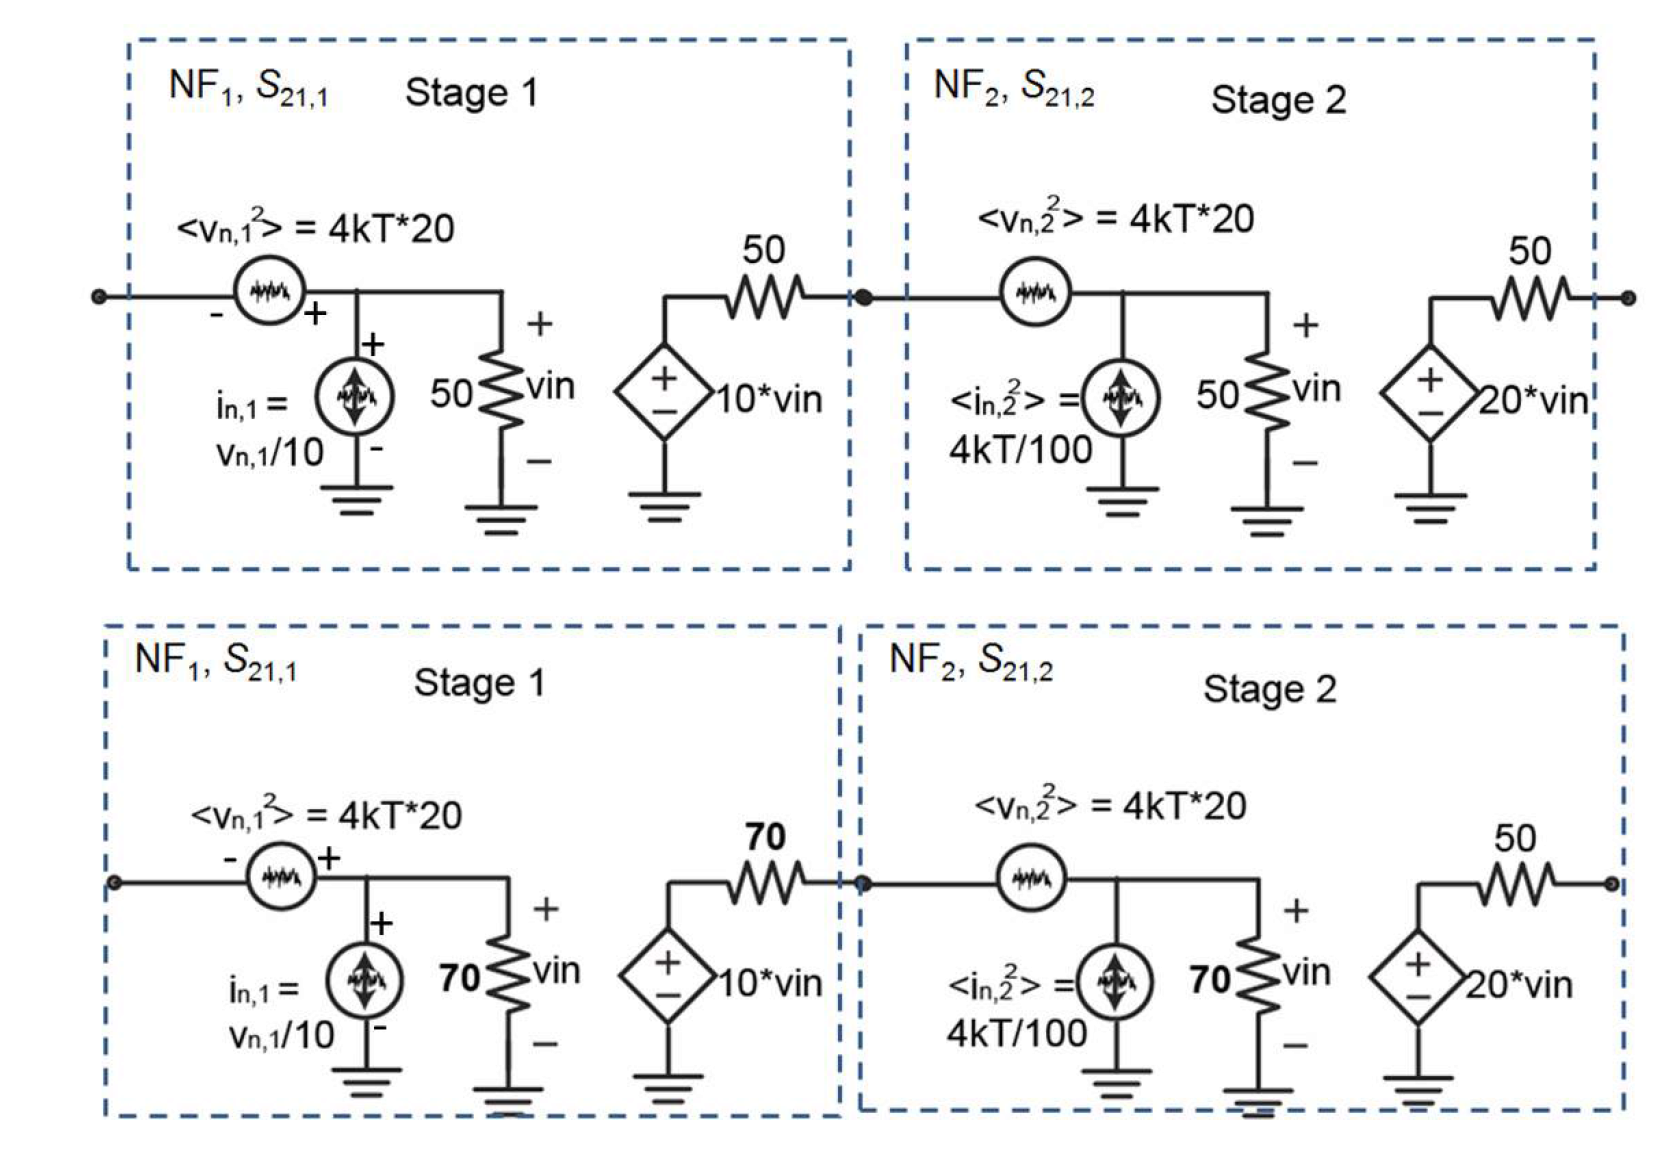
\includegraphics[width=\textwidth-2cm]{problem1a_schematic.png}
    \end{figure}

    \item {\color{blue}For the above two cascade circuits, calculate the power gains and noise figures for each stage (i.e. $S_{21,1}$, $S_{21,2}$, $NF_1$, $NF_2$) and the two stage circuits ($S_{21,total}$, $NF_{total}$).
    The resistors are assumed to be noiseless.}

    \subsection{Cascade 1 - S}
    \begin{align*}
        S_{21,1} &= 5 \\
        S_{21,2} &= 10 \\
        S_{21,total} &= 50
    \end{align*}

    We assumed $Z_0$ is $50 \Omega$. We drive the input with a 50 $\Omega$ AC source and terminate the output with a $50 \Omega$ load.
    These values represent voltage and power gain due to equal input/output impedances.

    \subsection{Cascade 1 - Noise}

    For the first cascase's stage 1, we begin by input referring the noise sources and collapsing the voltage and current noise into $\overline{v_{eq}^2}$.
    From lecture:

    \begin{align*}
        \overline{v_{eq}^2} &= \overline{v_n^2} + \overline{i_n^2} R_s^2 \text{ for uncorrelated noise} \\
        \overline{v_{eq}^2} &= \overline{v_n^2} |1 + Y_c Z_s|^2 + |Z_s|^2 \overline{i_u^2} \text{ for correlated noise} \\
        \text{ where } i_c &= Y_c V_n \text{ and } i_n = i_c + i_u \\
        \text{ then } F &= 1 + \frac{N_{amp,i}}{N_s} = 1 + \frac{\overline{v_{eq}^2}}{\overline{v_s^2}}
    \end{align*}

    Assume we are calculating noise figure in a $50 \Omega$ environment, $R_s = 50 \Omega$ and $\overline{v_s^2} = 4 kT R_s$.
    We assume that all noise sources represented are defined as \emph{spot noise}.
    Furthermore, we \emph{don't} assume that $\overline{v_n^2}$ and $\overline{i_n^2}$ are uncorrelated, and include covariance terms when needed.

    \begin{align*}
        F_1 &= 1 + \frac{\overline{v_{eq,1}^2}}{\overline{v_s^2}} = 1 + \frac{4kT\cdot 20 |1 + 0.1 \cdot 50|^2}{4kT \cdot 50} = 15.4 \\
        NF_1 &= 10 \cdot \log(F_1) = 11.88 \text{ dB} \\
        F_2 &= 1 + \frac{\overline{v_{eq,1}^2}}{\overline{v_s^2}} = 1 + \frac{4kT \cdot 20 + 4kT \cdot \frac{1}{100} \cdot 50^2}{4kT \cdot 50} = 1.9 \\
        NF_2 &= 2.79 \text{ dB} \\
        F_{tot} &= F_1 + \frac{F_2 - 1}{G_1} = 15.4 + \frac{1.9-1}{5^2} = 15.436 \\
        NF_{tot} &= 11.885 \text{ dB}
    \end{align*}

    where we recognize that all current noise is correlated to the voltage noise. Furthermore, we can use Friis' cascade noise formula due to internally matched impedances.

    \subsection{Cascase 2 -S}
    \begin{align*}
        S_{21,1} &= \frac{V_s \frac{70}{70 + 50} \cdot 10 \cdot \frac{50}{50 + 70}}{V_s \frac{70}{70+50}} = 4.147 \\
        S_{21,2} &= \frac{V_s \frac{70}{70 + 50} \cdot 20 \cdot \frac{1}{2}}{V_s \frac{70}{70+50}} = 10 \\
        S_{21,total} &= \frac{V_s \frac{70}{70+50} \cdot 10 \cdot \frac{1}{2} \cdot 20 \frac{1}{2}}{V_s \frac{70}{70+50}} = 50
    \end{align*}

    \subsection{Cascase 2 - Noise}
    \begin{align*}
        F_1 &= 15.4 \text{ same as cascase 1} \\
        F_2 &= 1.9 \text{ same as cascase 1} \\
        F_{tot} &= 15.436
    \end{align*}

    The noise figure of each stage doesn't change because input referring the noise sources doesn't depend on the stages' terminations. The total noise figure also doesn't change since input referring the noise from the second stage still sees a pure gain by 10.

    \item {\color{blue} Is the formula $NF_{total} = NF_1 + \frac{NF_2-1}{|S_{21,1}^2|}$ applicable?}

    This formula is definetely applicable if each stage is impedance matched internally and to the external source resistance and load impedance used in the measurement; otherwise it doesn't apply generally.

    \item {\color{blue} For a lossy transmission line illustrated below, derive its noise figure.}

    \begin{figure}[H]
        \centering 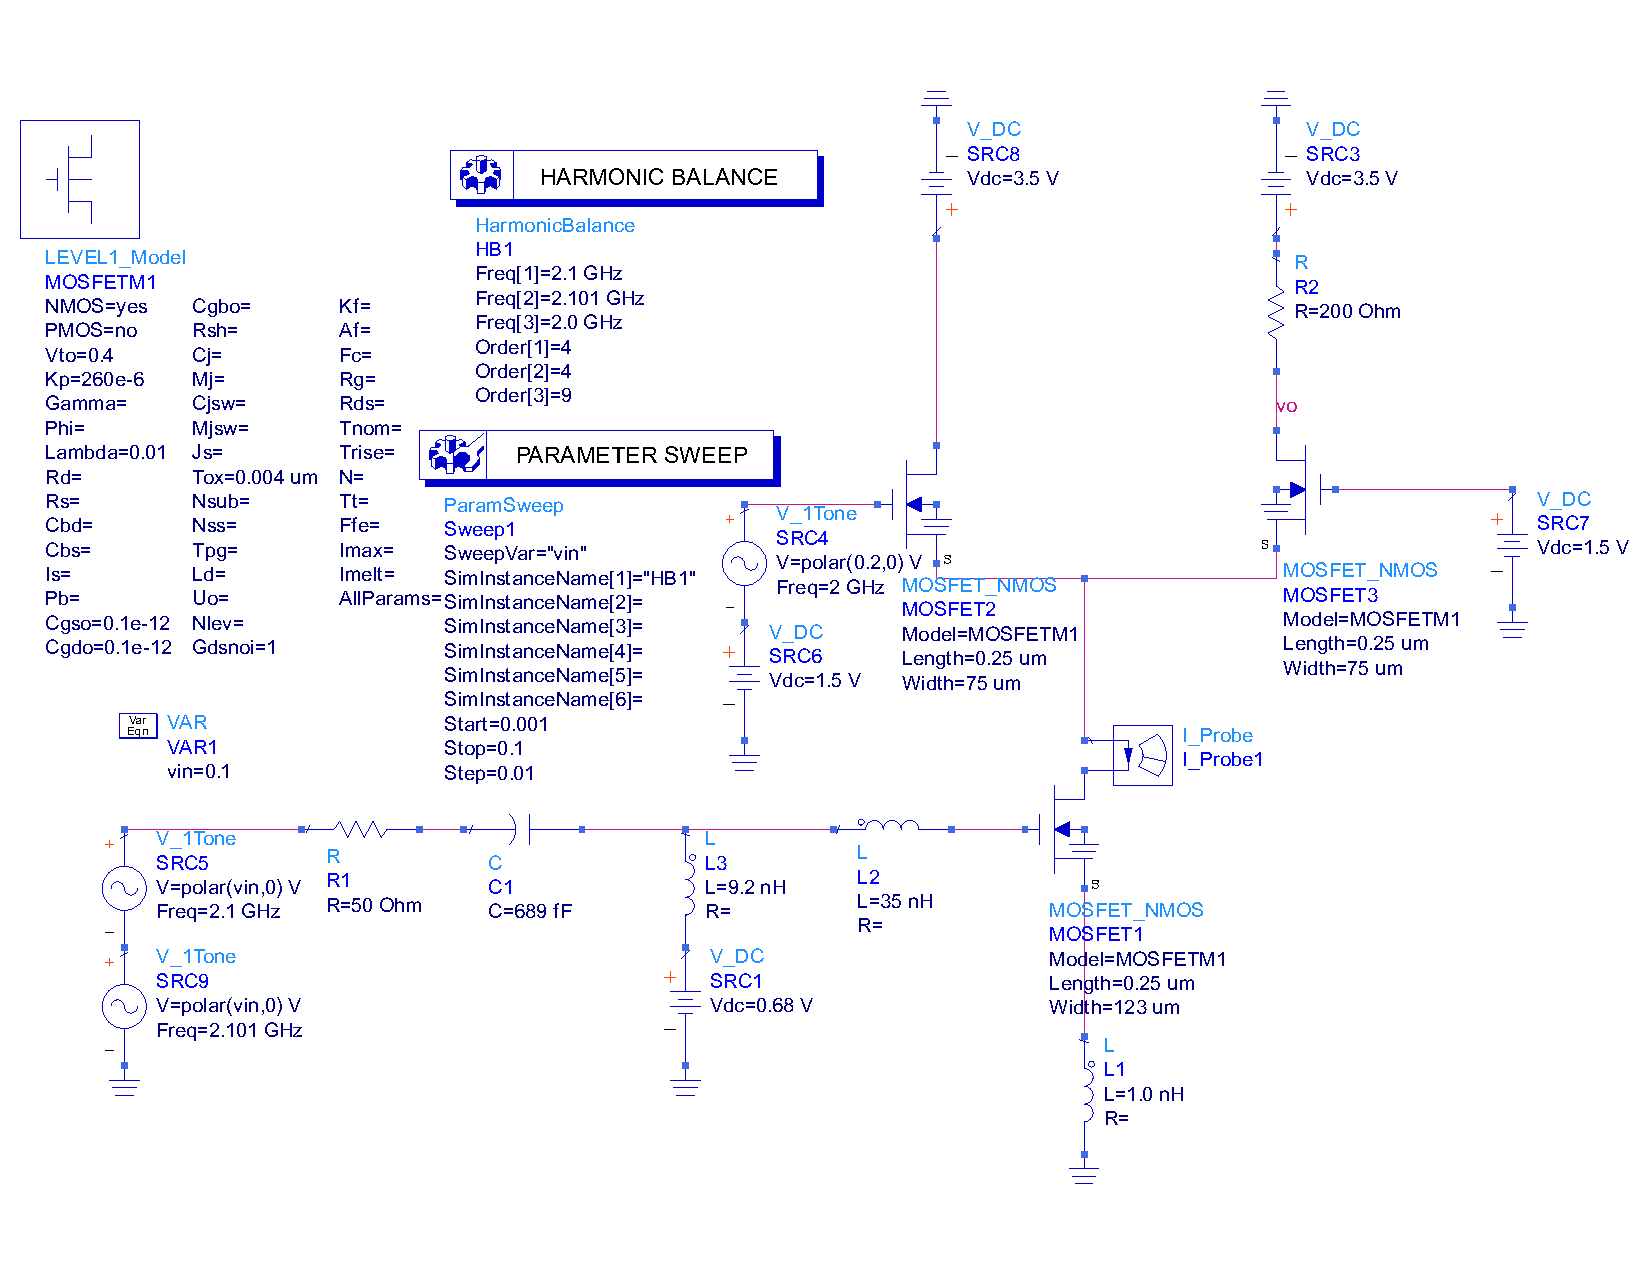
\includegraphics[width=\textwidth-8cm]{problem1c_schematic.png}
    \end{figure}

    Starting with the definition of $F$:

    \begin{align*}
        F &= \frac{SNR_i}{SNR_o} = \frac{P_{sig}/\overline{v_{n,s}^2}}{P_{sig} \cdot \text{ loss} / \overline{v_{n,s}^2} \cdot \text{ loss}^2} \\
        F &= \frac{1}{\text{loss}}
    \end{align*}

    where 'loss' represents the power loss of the transmission line in steady state from input to output. This is simple to compute, assuming that the line is driven with a source impedance of $Z_0$ with a mean squared noise voltage of $4 kT Z_0$ and terminated with a noiseless load of $Z_0$.

    \begin{align*}
        \text{Power @ Load} &= V_+ e^{-\gamma l} \cdot \frac{1}{Z_0} e^{-\gamma l} V_+ \rvert_{l=0} = \frac{V_+^2}{Z_0} \\
        \text{Power @ Source} &= V_+ e^{-\gamma l} \cdot \frac{1}{Z_0} e^{-\gamma l} V_+ \rvert_{l=-l} = \frac{V_+^2 e^{2 \gamma l}}{Z_0} \\
        \text{Power @ Load / Power @ Source} &= e^{-2 \gamma l} \\
        F &= \frac{1}{e^{-2 \gamma l}} = e^{2 \gamma l}
    \end{align*}

    We know the propagation constant $\gamma = \alpha + j \beta$. Because the velocity of the line is at the speed of light, the imaginary term goes to zero and $\gamma$ is dominated by $\alpha$.

    $$ F = e^{2 \alpha_0 L} $$

    The noise figure seems frequency independent, but any real line has $\beta = \frac{2\pi}{\lambda}$.

    \item {\color{blue} If the tline is used to connect the above two cascade circuits to the $50\Omega$ soucrce (e.g. antenna), what will be the new total noise figures}
\end{enumerate}

\section{Matching for Low Noise Versus Matching for High Gain}
\emph{In this problem, your answers should be functions of frequency.}

\begin{enumerate}[label=(\alph*)]
    \item {\color{blue} For a simplified common-source model shown below (with noise sources drawn) derive the input referred noise voltage and noise current.}
\end{enumerate}
\end{document}
